
%-----------------------------------------------------------------------------
\chapter{SnpEff: Genomic variant annotation and prioritization\label{ch:snpeff}}
%-----------------------------------------------------------------------------

%---
\section{Preface}
%---

As this thesis is focused on extracting biological insight from sequencing data, in this chapter we examine algorithms we created for calculating ``functional annotations" of genomic variants. In essence, functional variant annotations are bits of biological knowledge that allow us to make prioritize variants that are assumed to be more relevant to the phenotypic trait under study and to filter out variants assumed irrelevant. The spectrum of functional annotations for a genomic variant is wide and may involve information on which genes are affected by the variant, how the protein product is affected, how conserved is the genomic region the variant lies onto, and which clinically relevant information is associated with the loci; just to mention a few typical use cases.

When trying to find variants that affect risk of complex disease, statistical power is paramount. We need to be able to ``separate wheat from chaff". In our context this means two different but closely related tasks: i) performing functional annotations, and ii) using that information for prioritizing variants (and filtering out the ones we suspect are not related to the particular trait under study). Failing to efficiently filter out irrelevant variants would reduce our statistical power as more statistical tests are calculated, thus would decrease our chances of finding the associations we are looking for. In order to efficiently annotate and filter variants, we created two software packages called SnpEff and SnpSift that deal with the annotation and filtering aspects respectively.

%---
\section{Epilogue?}
%---

At the beginning of my Ph.D., functional annotation of genomic variants was an unsolved problem with many research labs creating in-house custom solutions that oftentimes were inefficient and lacking of rigorous testing. As a consequence, shortly after SnpEff \& SnpSift were released they quickly became widely adopted by the research community as well as many private organizations. Currently SnpEff \& SnpSift has over 250 downloads per week (as reported by  SourceForge, where the tools are hosted). So far SnpEff \& SnpSift  have been cited over 400 times.

\subsection{Data structures for annotations}

A very simple approach used by ANNOVAR \cite{wang2010annovar} is to create an index by dividing each chromosome into $N$ bins of equal size. All genomic features are stored in a hash table indexed by chromosome name and bin number. This approach has running time of $O(n)$ where $n$ is the number of features, but it can be easily tuned by creating small bins, at the cost of increased memory requirements.

Another approach \cite{cingolani2012program} is to use an ``interval forest'', which is a hash of ``interval trees'' indexed by chromosome. Each interval tree is composed of nodes. Each node has five elements i) a center point, ii) a pointer to a node having all intervals to the left of the center, iii) a pointer to a node having all intervals to the right of the center, iv) all intervals overlapping the center point sorted by start position, and v) all interval overlapping the center point sorted by end position. Querying an interval tree requires $O[log(n) + m]$ time, where $n$ is the number of features in the tree and $m$ is the number of features in the result. Having a hash of trees optimizes the search by reducing the number of intervals per tree.


%---
\section{Background}
%---

The development of cost-effective, high-throughput next generation sequencing (NGS) technologies is poised to have a profound impact on our ability to study the effects of individual genetic variants on the pathogenesis and progression of both monogenic and common polygenic diseases. As sequencing costs decrease and throughput increases, it has now become possible to quickly identify a large number of sequence polymorphisms (SNVs, indels, structural) using samples from affected and unaffected subjects and investigate these in epidemiologic studies to identify genomic regions where mutations increase disease risk. However, translating this information into biological or clinical insights is challenging as it is often difficult to determine which specific polymorphisms are the main pathogenetic drivers of disease across a population; and more importantly, how they affect the activity of disease-related molecular pathways in tissues and organism a specific patient. In part, this difficulty results from the large number of genetic variants that are observed in individual genomes (the human population is believed to contain approximately 3.5 million polymorphic sites with minor allele frequency above 5\%) combined with the limited ability of computational approaches to distinguish variants with no impact on genome function (the vast majority) from variants affecting gene function or expression that may be associated with disease risk or drug response (the minority). The development of algorithms for automated variant annotation,which link each variant with information that may help predict its molecular and phenotypic impact, is a critical step towards prioritizing variants that may have a functional impact from those that are harmless or have irrelevant functional effects. The goal of this protocol is to collect relevant information that will help answer questions about genetic variants discovered in next-generation sequencing studies, including: (i) will a given coding variant affect the ability of a protein to carry its functions; (ii) will a given non-coding variant affect the expression or processing of a given gene; and ultimately (iii) will a given coding or noncoding variant have any impact on phenotypes of interest?

Answering these questions is essential for many types of analyses that use large-scale genomics datasets to study quantitative traits and diseases, particularly when only a small number of individuals is studied comprehensively at a genome-wide level. For example, most genome-wide association studies (GWAS) or exome sequencing studies lack the statistical power to identify rare variants or variants with small effects associated with a disease, in part due to the large number of variants assayed. This limitation can be addressed by directing subsequent experimental steps to focus on smaller sets of genetic variants that have been prioritized based on external evidence of their putative impact. The common impairment of DNA repair mechanisms and chromatin stability in malignant cells leads to a similar challenge in cancer genomics, where the hundreds or thousands of mutations that distinguish an individual’s tumor and germline genomes need to be classified on the basis of their putative phenotypic effects and potential roles in carcinogenesis.

The large number of databases containing potentially helpful information about a given variant make the process of gathering and presenting relevant data challenging, despite excellent tools that already exist to analyze large genomics datasets (including GATK \cite{mckenna2010genome} and Galaxy \cite{goecks2010galaxy}) and visualize the results (such as the UCSC \cite{karolchik2014ucsc} or Ensembl \cite{flicek2012ensembl} genome browsers). Each of these databases uses its own format and is updated asynchronously, which makes it difficult for any analysis to remain up to date. In addition, the lack of comprehensive and computationally efficient models that allow integrative analyses using these resources, makes the task of comprehensive variant annotation overwhelming. By efficiently combining information from tens or hundreds of genome-wide databases, the tools and protocol described here are designed to greatly facilitate the process of variant annotation, and make it accessible to groups with limited bioinformatics expertise or resources.

In this protocol, we describe an approach to variant annotation that automatically collects, integrates, and presents a wide body of publicly available evidence of functional impact of a given set of genomic variants. The pipeline, based on the SnpEff package \cite{cingolani2012program}, is easy to execute and efficiently extracts a comprehensive set of variant annotations that can be used to prioritize downstream clinical or functional studies. SnpEff is used in many large genome centers and supports variant annotation for thousands of species, although the extent and quality of annotations extracted for a set of variants depends on the amount of publicly available genomics data for that species. In the case of whole-genome or exome sequences from human DNA samples, SnpEff extracts metadata (annotations) for each variant from relevant sources including gene annotation data identifying transcribed and translated regions; estimates of the frequency with which each variant occurs in different populations (from the 1000 Genomes project and the Exome Sequencing project \cite{10002012integrated}); and data that describes the function of regulatory elements that may be altered by the variant (obtained from the ENCODE project \cite{encode2012integrated} and Epigenome Roadmap \cite{bernstein2010nih}). SnpEff allows flexible and efficient querying of these annotations and is sufficiently fast to analyze very large sets of variants on a small computer (see Box 1 for computational and algorithmic considerations). It is also able to detect and be robust to a variety of gene annotation inconsistencies that would otherwise trigger false-positive high-impact variant predictions. In addition to SnpEff, an number of other annotation packages have been developed (including ANNOVAR \cite{wang2010annovar}, the Ensembl Variant Effect Predictor \cite{mclaren2010deriving}, GEMINI \cite{paila2013gemini} and VAT \cite{habegger2012vat}), which differ in terms of their functionality, ease-of-use, computational efficiency, and robustness.

%---
\section{Genetic variants}
%---

For most species, genetic variants are identified by comparing genome sequences from an individual organism to a reference (haploid) genome (see Box 2). A genetic variant, at a specific location in the genome (genetic locus) can be represented by agenotype which describes the difference between the DNA sequence present on each chromosome in the individual’s diploid genome and the reference genome. At a specific polymorphic locus, an individual can thus be homozygous for the reference allele, heterozygous, or homozygous for the non-reference allele.

There are as many types of genetic variants as there are types of mutations, and their frequency and breadth of impact on the genome vary tremendously \cite{ng2009targeted}. The most common type of variant identified by current technologies and analysis approaches is a single base difference with respect to the reference genome. Depending on whether the variant was identified in an individual or in a population, it is called a Single Nucleotide Variant (SNV) or Single Nucleotide Polymorphism (SNP). Sequence differences affecting several consecutive nucleotides are called a multiple nucleotide polymorphism (MNP) and are typically treated as a single variant locus if they are in perfect linkage disequilibrium. Short insertions and deletions (indels) of a chromosome region range from 1 to 20 bases in length are approximately 30 times less frequent than SNVs1but may have profound effects on protein activity by altering the translation reading frame or deleting a protein domain. Genomic variants involving larger regions are more rare and more difficult to infer using short-read NGS technologies. Those include large deletions, which can result in the loss of an exon or one or more whole genes, and insertions, which often originate from transposable elements or tandem duplications. Large genome variants that cause the number of copies of a particular genomic region to be polymorphic in a population are called a Copy Number Variants (CNV). Genomic rearrangements such as inversions and translocations are events that involve two or more genomic breakpoints and a reorganization of genomic segments, possibly resulting in gene fusions or loss of critical regulatory elements. This protocol does not address the annotation or rearrangements due to the challenges involved in their identification and functional characterization and their relative rarity in the germ line.

The process of inferring variants present in an individual’s genome from sequencing data is called variant calling and is based on sophisticated algorithms that have been reviewed elsewhere \cite{nielsen2011genotype}. Genome-wide variant calling has until recently largely been done using genotyping arrays (for SNVs) or Comparative Genomic Hybridization arrays (for CNVs). The inherent limitations of these technologies, particularly their ability to only assay genotypes at sites that are known in advance to be polymorphic, combined with the declining cost of sequencing, have now made approaches based on high-throughput resequencing the tool of choice for variant calling in clinical studies. Although this is a challenging task and remains an important area of research, many high-quality tools exist for calling SNVs and indels (such as GATK2 and SamTools \cite{li2009sequence}), as well as detecting CNVs (such as PennCNV \cite{wang2007penncnv} and CNVhap \cite{coin2010cnvhap}), and structural variants (e.g. VariationHunter \cite{hormozdiari2011simultaneous}). The output of these tools – variant calls – are stored using the standardized format called the Variant Call Format \cite{danecek2011variant} (VCF; see Box 3). Their calling accuracy depends on the type of variants, their frequency in the population of patients or tumor cells being studied, and the quantity (coverage) and quality of the sequencing data. As the length, accuracy and coverage of sequencing reads increases, variant calling will become easier and more accurate. Therefore, we discuss here the problem of annotating the variants identified by some of these tools, and refer the reader to the review by Nielsenet al.14 to learn more about the process of variant calling itself.

\subsection{Types of genetic annotations}

The process of genetic variant annotation consists of the collection, integration, and presentation of experimental and computational evidence that may shed light on the impact of each variant on gene or protein activity and ultimately on disease risk or other phenotypes. Variant annotation has traditionally been divided in two apparently independent but actually interrelated tasks based on the variant’s location with respect to known protein-coding genes (see Table 1 for a list of commonly used variant annotations).Coding variant annotation focuses on variants that are located within coding regions of annotated protein-coding genes and attempts to assess their impact on the function of the encoded protein. In contrast,non-coding variant annotation focuses on variants located outside the coding portion of genes (i.e. in intergenic regions, UTRs, introns, or non-protein-coding genes) and aims to assess their potential impact on transcriptional and post-transcriptional gene regulation. These two categories of variant annotations are not mutually exclusive, as variants located within exons can often have an impact on the gene transcript’s processing (splicing). In addition, some transcripts can have both protein-coding and non-coding functions. Despite the intermingling of the notion of coding and noncoding variants, we will consider each type of annotation separately as assessing their impact requires different sources of data and algorithms.

The ultimate goal of variant annotation is to predict the impact of a sequence variant, although this is an ill-defined term. One the one hand, one may be interested in the molecular impact of a variant on the activity of a protein. On the other, others may be interested in a variant’s impact on much higher-level phenotypes such as disease risk. Mutations that are predicted to completely abrogate a gene’s activity are calledloss-of-function (LOF) mutations; while mutations that are tentatively predicted to have less severe consequences are called moderate or low impact mutations.In practice, a variant will be predicted to cause LOF if it has two properties: (i) its molecular impact is reliably predictable by existing computational approaches (e.g. gain of stop-codon); and (ii) its functional impact, reflected by altered protein activity or expression levels, is expected to be large. Many types of variants, including most non-coding variants, may have a large functional impact but lack predictability, and as a consequence are typically not predicted to be LOF variants.

\subsection{Coding variant annotation}

Coding variants occur in a translated exon. When a reliable gene annotation is available, their main impact can be classified by determining their effect on the translated amino acid sequence (if any). A synonymous coding variant (also called silent) does not change the sequence of amino acids encoded by the gene, although it may impact aspects of post-transcriptional regulation such as splicing and translation efficiency and can affect the total protein activity through changes in the amount of translated protein that is made in the cell. In contrast, a non-synonymous coding variant changes one or more amino acids encoded by the gene and can directly alter the protein’s activity, localization or stability. Non-synonymous variants include missense substitutions that change a single amino acid, nonsense substitutions that lead to the gain of a stop codon,frame-preserving indels that insert or delete one or more amino acids, and frame-shifting indels that may completely alter the protein’s amino acid sequence. Primary annotation and assessment of impact, which performed directly by SnpEff, determines whether a variant falls in any of these categories.

\textbf{Caveats}
	\begin{enumerate}[label=\roman*]
	
	\item \textit{Gene misannotation.} Genomic variants that have a significant effect on a protein’s expression or function represent a very small fraction of all variants. Assembly and gene annotation errors or genomic oddities that break classical computational models are also rare, but often overestimate the variant’s impact. This implies that one is likely to find a non-negligible fraction of false-positive high-impact variants among the list of what appear to be the strongest candidates for variants with severe effects. Tools such as SnpEff can anticipate some of the most common causes of misannotation, but the number and diversity of the type of events that can lead to false-positives makes the task very challenging. As a consequence, one should always manually inspect the top candidates to ensure that they have been assigned to the correct genes and transcripts.
	
	\item \textit{Gene isoforms.} In higher eukaryotes, most genes have more than one transcript (or isoform), due to alternative promoters, splicing, or polyadenylation sites. For example, a human gene has an average of 8.8 annotated messenger RNA (mRNA) isoforms and some genes are believed to have over 4,000 isoforms resulting from complex splicing programs. For these genes, a variant may be coding with respect to one mRNA isoform and non-coding with respect to another. There are two frequent approaches to address this situation: (i) annotate a variant using the most severe functional effect predicted for at least one mRNA isoform; or (ii) use only a single canonical transcript per gene to perform primary annotation. 
	
	\item \textit{Variant calling for indels.} Variant annotation relies on knowing the exact genomic coordinates of the variant: this is rarely a problem for isolated SNVs; however, insertions and deletions often cannot be located unambiguously. Consider for example the variant $AA \rightarrow A$. This mutation results in the loss of a single base, but was it the first or second A that was deleted? From the standpoint of the cell, this question is irrelevant and deletion of any A will have the same effect. In contrast, from the standpoint of most variant annotation software, deleting the first A is different from deleting the second. Consider the scenario of a previously annotated transcript where the first A is part of the 5' UTR and the second is the first base of a start codon. If the missing base is assigned to the leftmost position in the motif (as is the current convention), the deletion would be annotated as a low impact 5'UTR variant. However, assigning it to the rightmost A would make it appear (incorrectly) to be a high-impact start-codon deletion. Similar issues may arise when considering conservation scores or transcription factor binding site (TFBS) predictions.
	
		\end{enumerate}

\subsection{Loss of function variants}

True LOF variants are difficult to predict computationally, but specific types of genetic changes will frequently lead to severely impaired protein activity. These include (i) stop-gains (nonsense mutations) and start-loss; (ii) indels causing frameshifts; (iii) large deletions that remove either the first exon or at least 50\% of the protein coding sequence; and (iv) loss of splice acceptor or donor sites that alter the protein-coding sequence. Variants that introduce premature in-frame stop codons (nonsense mutations and most frameshift indels) are expected to abolish protein function, unless the variant is very near the C-terminus of the coding region \cite{yamaguchi2008distribution} (effectively, downstream of the last functional domain in the protein). This may cause severe consequences in affected cells, tissues or organism, as is seen for mutations that cause monogenic diseases \cite{scheper2007translation}. In addition, a new stop codon that lies upstream of the last exon will likely trigger nonsense mediated decay (NMD), a process that degrades mRNA before protein synthesis occurs \cite{nagy1998rule}. NMD predictions are not exact and many factors can affect mRNA degradation, including the variant’s distance from the last exon-exon junction or poly-A tail, and the possibility that transcription may re-initiate downstream of the LOF variant \cite{brogna2009nonsense}.

A variant that leads to the loss of a stop codon, sometimes called aread-through mutation, will result in an elongated protein-coding transcript that terminates at the next in-frame stop codon. While there are no general models that predict how deleterious this may be, variants that elongate the reading frame can also result in aberrant folding and degradation of the nascent proteins, leading to activation of cellular stress response pathways in addition to their direct effects on protein activity and expression levels21.

The effect of the loss of a start codon depends on the location of a replacement start codon with respect to the translation start site and reading frame of the native protein. If the new start codon maintains the reading frame, the only consequence may be the loss of a few amino acids in the protein transcript; however, in many cases, the new start codon will not be in-frame, thus producing a frame-shifted protein that is later degraded. In addition, the new start codon may lack an appropriate regulatory context (for example, if there is no Kozak sequence nearby or if it disrupts 5’ UTR folding) leading to reduced expression of an N-terminally truncated protein. Consequently, losing a start codon is thought to be highly deleterious in most cases, due to the potential that it may reduce both protein production and activity.

\textbf{Caveats}
	\begin{enumerate}[label=\roman*]
	
	\item \textit{Rare amino acids.} Through a process called translational recoding, a UGA ``Stop" codon located in the appropriate mRNA context (determined by both primary mRNA sequence and secondary structure) may be translated to incorporate a selenocysteine amino acid (Sec / U). In humans, this occurs at approximately 100 codons located in mRNAs whose 3’ UTR contains a Selenocysteine insertion sequence element (SECIS). Since the translation machinery goes so far to encode these special rare amino acids, the expectation is that mutations at those sites would be highly deleterious. This is supported by evidence that reduced efficiency of selenocysteine incorporation is linked to severe clinical outcomes, such as early onset myopathy  \cite{maiti2009mutation} and progressive cerebral atrophy  \cite{agamy2010mutations}.
	
	\item \textit{False-positives in LOF predictions.} Variants predicted to result in a LOF sometimes actually produce proteins that are partially functional  \cite{macarthur2012systematic}. In fact, an apparently healthy individual is typically heterozygous for around 100 predicted LOF variants, and homozygous for roughly 10 variants, but many of those are unlikely to completely abolish the protein function. Indeed, these variants are enriched toward the 3’ end of the gene, where they are likely to be less deleterious. 
	
	\end{enumerate}

\subsection{Variants with low or moderate impact}

Compared to the high impact variants discussed above, where extensive prior biological evidence strongly suggests that a specific type of variant will severely impair protein activity, there are few guidelines that can reliably predict how the majority of nonsynonymous (missense) variants will alter protein function or expression. As a result, the primary annotation performed by SnpEff and most related software packages will broadly categorize missense substitutions and their accompanying amino acid changes (e.g. K154->L154) as moderate impact variants. Short indels whose length is a multiple of three are treated similarly, unless they introduce a stop codon, as their effect will usually be localized.

Once missense and frame-preserving indel variants are identified, a more detailed estimation of their impact on protein function can be performed using heuristic and statistical models. The most common approaches are based on conservation, either amongst orthologous or homologous proteins, or protein domains, sometimes adding information of the physio-chemical properties of the reference and variant amino acids (e.g. differences in side chain charge, hydrophobicity, or size). The SIFT algorithm \cite{kumar2009predicting} assesses the degree of selection against specific amino acid changes at a given position of a protein sequence by analyzing the substitution process at that site throughout a collection of predicted homologous proteins identified by PSI-BLAST \cite{altschul1997gapped}. Based on this multiple sequence alignment and the highly conserved regions it contains, SIFT calculates a normalized probability of amino acid replacement (called the SIFT score), which estimates the mutation’s effect on protein function.Polyphen \cite{adzhubei2010method}, another commonly used tool, takes the process one step further by searching UniProtKB/Swiss-Prot \cite{uniprot2013update} and the DSSP database of secondary structure assignments \cite{joosten2011series} to determine if the variant is located in a known active site in the protein.In contrast to other methods that categorize each variant individually, VAAST \cite{rope2011using}, a commercially available package, computes scores for groups of variants located within a given gene and ``collapses" them into a single category, a concept similar to burden testing performed for rare variants identified in exome sequencing studies.For human proteins, SnpEff makes use of the Database for Nonsynonymous SNVs’ Functional Predictions \cite{liu2011dbnsfp} (dbNSFP), which collects scores produced by several impact assessment algorithms in a single database. Individually, impact assessment methods usually have an estimated accuracy of 60\% to 80\%, but predictions from several algorithms can be combined to provide a stringent, but more accurate estimate of impact \cite{choi2012predicting}.

In most cases these algorithms apply best to SNVs since these are common in populations and there is more genomic sequence andexperimental data available to refine the statistical methods. However, some recently developed algorithms are capable of assessing variants other than SNVs, including PROVEAN \cite{choi2012predicting}, which extends SIFT to assess the functional impact of indels.

\textbf{Caveats}
	\begin{enumerate}[label=\roman*]
	
	\item \textit{Imprecise models of protein function.} Accurate impact assessment of coding variants remains an open problem and most computational predictions are riddled with both false positives and false negatives. While both missense variants and frame-preserving indels are broadly cataloged as having moderate effects, this is mostly due to lack of a comprehensive model and the extremely complex computations that would be required for an in-depth analysis (such as protein structure predictions). In these cases, proteomic information can be revealing. SnpEff adds annotations from curated proteomic databases, such as NextProt  \cite{lane2012nextprot}, which can help to elucidate if a mutation alters a critical protein amino acid or domain (such as amino acids that are post-translationally modified as part of a signaling cascade or that are form the active site of an enzyme) resulting in a protein may no longer function.
	
	\item \textit{Gain of deleterious function.} Computational variant annotation may eventually be able to fairly accurately predict the molecular impact of a variant in terms of the degree to which it translates in a loss of function for the encoded protein. However, gains of function, including the acquired ability to interact with new partners and disrupt their function, remain vastly more difficult to tackle, although a several such variants have been linked to disease, such as hereditary pancreatitis  \cite{whitcomb1996hereditary}.
	
	\item \textit{Unanticipated effects of synonymous variants.} In most cases, synonymous variants are regarded as non-deleterious (or low impact); however, one needs to seriously consider the possibility that they may have greater functional effects by altering mRNA splicing  \cite{coulombe2009fine} or secondary structure  \cite{sabarinathan2013rnasnp}. Synonymous SNVs may also alter translation efficiency, by changing a frequently used to a rarely used codon and have been linked to changes in protein expression  \cite{sauna2011understanding}.
	
	\end{enumerate}

\subsection{Non-coding variant annotation}

Although coding variants represent less than 2\% of variants in the human genome, they make up the vast majority of confirmed disease-related variants that have been validated at a functional level. This may result from ascertainment bias (since variants in coding regions are straightforward to discover and characterize at a basic level and many studies have largely ignored non-coding variants); or may be explained by the increased complexity of computational approaches and lab assays required to predict and validate the impact of non-coding variants; or by their potentially more subtle impact on gene expression or cell function. Nonetheless, in a compendium of current GWAS studies, roughly 40\% of the variants are intergenic and 30\% intronic and functional studies of these variants are increasingly emphasizing the importance of non-coding genetic variation at risk loci for complex genetic diseases and traits \cite{hindorff2009potential}.

Functional non-coding regions of the genome encompass a wide variety of regulatory elements contained in DNA and RNA molecules that are involved in transcriptional and post-transcriptional regulation. Cis-regulatory elements include (i) binding sites for DNA-binding proteins such as transcription factors and chromatin remodelers; (ii) binding sites for RNA-binding proteins involved in splicing, mRNA localization, or translational regulation; (iii) micro RNA (miRNA) target sites; and (iv) long non-coding RNA (lncRNA) targets on DNA, RNA and proteins. Non-coding transcripts include well-characterized regulatory RNAs (e.g. miRNA, snoRNA, snRNA, piRNA and lncRNAs) as well as RNAs involved directly in protein synthesis (e.g. tRNA and rRNA).  The annotation and impact assessment of non-coding variants presents a significant challenge for several reasons: (i) reliable technologies to study transcriptional regulatory regions on a genome-wide basis are only just reaching maturity and provide limited resolution of binding sites for individual transcription factors and regulatory RNA molecules; (ii) non-coding functional regions of most genomes remain incompletely mapped as they vary widely among different cell types and cell states (for example, in diseased and healthy tissues); (iii) non-coding regulatory elements often are part of complex transcriptional programs that are time-dependent, contain many redundant linkages or reciprocal connections between genes and respond to a wide range of intra- and extracellular signals; and (iv) genomic regulatory elements rarely have a strict consensus sequence (for example, compare the position weight matrices used to identify transcription factor or miRNA binding sites with the amino acid triplet code) making the effect of a mutation on gene regulatory programs difficult to predict. As a result, high-quality annotation of non-coding variants relies more heavily on experimental data than is the case for coding variants: since many of these experimental techniques did not study the effects of SNVs on gene regulatory programs, they can only be used to annotate variants and not to predict their effects on gene transcription. In the few cases where the effects of SNVs have been studied (for example, the effects of SNVs that are common in a population and located in genetic loci associated with complex diseases), experimental approaches provide highly accurate functional assessment at a cost of reduced coverage compared to computational approaches.

Large-scale projects such as ENCODE7and modENCODE \cite{celniker2009unlocking} have made major steps toward mapping gene transcription and transcriptional regulatory regions in many tissues and cell types, but similar studies in diseased tissues remain at an early stage (for example, the growing collection of disease-related epigenomes from the Epigenome Roadmap8). The base-by-base resolution and number of cell states studied for different types of regulatory elements and non-coding transcripts varies widely among datasets; in part due to the lack of sensitive, comprehensive and high-resolution technologies to study the different molecular species and modes of interaction that can be altered by non-coding variants. Efficient technologies for genome-wide, high-throughput mapping of binding sites for RNA-binding proteins (PAR-CLiP \cite{ascano2012identification}), miRNAs (PAR-CLiP \cite{hafner2012genome} and CLASH \cite{helwak2013mapping}) are starting to be applied on a broad scale as are protocols to map transcription factor binding sites (TFBS) which can improve resolution to a single base (Chip-exo \cite{rhee2012chip}). However, in most cases, DNA and RNA binding sites are only imprecisely located within Chip-Seq peaks that span genomic regions hundreds of base pairs in length, with computational approaches being used to pinpoint the bases most likely mediating the interaction. In the absence of more precise localization data,de novo computational prediction of binding sites for DNA and RNA binding proteins remains insufficiently accurate to be of much use in annotating single noncoding variants.

This limitation is particularly critical for functional predictions of putative target sites for microRNAs and other regulatory RNA species. MicroRNAs are short RNA molecules that regulate gene expression post-transcriptionally by binding the messenger RNA of a gene through complementary, usually in the 3’ region of the transcript, which leads to mRNA degradation or inhibits translation. Sequence variants that cause the loss or gain of a miRNA target site would lead to dysregulation of the gene, with likely deleterious effects. Although miRNAs are relatively well documented in most model organisms including human, their binding sites are only starting to be mapped experimentally, and computational predictions has very low specificity. Meaningful information regarding the possible role of a variant in disrupting a miRNA target site is starting to emerge \cite{liu2012mirsnp}, although variants that create new miRNA binding sites remain under the radar.

Even if the position of a functional element could be perfectly determined, predicting a variant’s impact on chromatin conformation, promoter activity, gene expression, or transcript processing remains challenging. For transcription factors, this involves predicting whether the protein will still be able to recognize its mutated site (and with what affinity), as well as predicting the impact of these changes on gene expression levels. The latter is particularly hard to predict as a result of interactions, competition, and redundancy contained in regulatory networks of transcription factors or RNA binding proteins. As a consequence, computational prediction of the functional impact of non-coding variants remains a very active area of research and there is no broad consensus on the best methodology to use \cite{ward2012interpreting}. One significant exception is the identification of variants affecting canonical splice sites, defined as two bases on the 3’ end on the intron (splice site acceptor) and 5’ end of the intron (splice site donor). Variants that affect canonical splice sites are easily detected and typically lead to abnormal mRNA processing, involving exon loss or extension that leads to loss of function of the encoded protein.

\subsection{Impact assessment of non-coding variants}

Two broad classes of publicly available genome-wide datasets are commonly combined to assess the functional impact of non-coding genetic variants: (i) computational predictions of sequence conservation and sites involved in molecular interactions such as transcription factor and RBP binding, as well as miRNA-mRNA target interactions; and (ii) experimental genome-wide localization assays for DNA binding proteins, histone modifications, and chromatin accessibility.

\paragraph{Computational sources of evidence:} Interspecies sequence conservation plays a key role in scoring and prioritizing non-coding variants. This is based on the assumption is that sites or regions that have been more conserved across species than expected under a neutral model of evolution are likely to be functional; suggesting that mutations contained in them are likely to be deleterious. In the absence of strong experimental data, sequence conservation measures calculated from whole genome multiple alignments, (for example using PhastCons  \cite{siepel2005evolutionarily}, SciPhy  \cite{garber2009identifying}, PhyloP  \cite{pollard2010detection} , and GERP  \cite{davydov2010identifying}), have been developed to provide a generic indicator of function for non-coding variants. Although high conservation scores generally mean that a genomic region may be functional, the converse is not true and many experimentally proven functional noncoding regions show only modest sequence conservation (for example due to binding site turnover events). Finally, some regulatory regions (e.g. specific elements regulating immune response  \cite{raj2013common}) are under positive selection and may thus show less conservation than surrounding neutral regions. 

In human, genome-wide computational predictions of transcription factor binding sites based on matching to publically available position weight matrices are available from variety of sources, including Ensembl 5 and Jaspar  \cite{bryne2008jaspar}.  Because of the low information content of most binding affinity profiles, the specificity of the predictions is generally very low. Related approaches exist to predict splicing regulatory regions  \cite{fairbrother2002predictive} and miRNA target sites \cite{ziebarth2011polymirts}, some of which are precomputed for whole genomes and available from the UCSC or Ensembl genome browsers. Recent efforts to determine RNA-binding protein sequence affinities can also be used to identify putative binding sites for these proteins in mRNA  \cite{ray2013compendium}.

\paragraph{Experimental sources of evidence:} To investigate the potential impact of variants on transcriptional regulation, many published experimental data sets produced by large-scale projects such as ENCODE 7, modENCODE 42 and Roadmap Epigenomics 8, can be used directly by annotation packages. These include: (i) ChIP-seq or ChIP-exo experiments that identify TFBSs on a genome-wide basis; (ii) DNAseI hypersensitivity or Formaldehyde-Assisted Isolation of Regulatory Elements (FAIRE) assays that identify regions with open chromatin; and (iii) ChIP-seq studies to identify the presence of specific promoter or enhancer-associated histone post-translational modifications, which can be combined to identify active, poised, and inactive enhancers and promoters 57. Most of these data sets are easily available through Galaxy 3 (as tracks from the UCSC Genome Browser) or through SnpEff (as downloadable pre-computed datasets). In parallel with the types of studies described above, expression quantitative trait loci (eQTLs) represent an agnostic way to map putative regulatory regions. An increasing number of such loci are available through the GTEX database  \cite{lonsdale2013genotype}. Experimental data that may support assessment of the impact of variants on post-transcriptional regulation remain sparser, although databases such as doRiNa  \cite{anders2011dorina} or starBase  \cite{yang2011starbase} contain genome-wide datasets obtained by CLIP-Seq and degradome sequencing. To our knowledge, these data have yet to be used in the context of variant annotation studies.

\paragraph{Combining sources of evidence:} Despite the variety of computational and experimental sources of evidence available, impact assessment for non-coding variants remains relatively crude, due to the fact that biological models of gene regulation remain fairly simple. Nonetheless, significant steps forward have been made recently, and two web-based tools, HaploReg  \cite{ward2012haploreg} and RegulomeDb  \cite{boyle2012annotation}, perform SNV and indel impact assessment for variants from dbSNV on the basis of a broad body of computational and experimental evidence. Both use pre-computed scores for variants from dbSnp and therefore cannot be used for rare variants, but they are extremely valuable for exploration by associating the variant of interest with a variant in dbSnp via linkage disequilibrium. 

\textbf{Caveats}
	\begin{enumerate}[label=\roman*]
	
	\item \textit{Sparseness of functional sites within ChIP-seq peaks.} Even if a noncoding variant is located in a region that contains a ChIP-seq peak for a given TF and has all the hallmark signatures of regulatory chromatin, the likelihood that it is deleterious remains low, because most DNA bases contained within a peak are non-functional. 
	
	\item \textit{Gain of function mutations.} While this section, has focused on variants causing the loss of a functional regulatory element, genetic variants may also create new or more effective transcription factor binding sites. These are substantially harder to detect as they can occur in regions that show no evidence of function in individuals possessing the reference allele, and show little conservation across species. Furthermore, computational methods to predict gain of affinity for a given TF caused by a variant have insufficient specificity to be of much use on their own. 
	
	\end{enumerate}

%---
\section{ Clinical effect of variants}
%---

One of the most revealing types of annotation of both coding and noncoding variants reports whether the variant has previously been implicated in a phenotype or disease. Although such information is available for only a small minority of all deleterious variants, their number is growing and should be the first type of annotation one seeks out. Clinical annotations, until recently, have been scattered in a large number of specialized databases of medical conditions with a genetic basis, including the comprehensive, manually curated collection of genetic loci, variants and phenotypes in the Online Mendelian Inheritance in Man database (OMIM, http://www.omim.org); web pages containing detailed clinical and genetic information about uncommon disorders in the Swedish National Board of Health and Welfare Database for Rare Diseases (http://www.socialstyrelsen.se/rarediseases) and the peer-reviewed NIH GeneReviews collection (54://www.ncbi.nlm.nih.gov/books/NBK1116); and a curated collection of over 140,000 mutations associated with common and rare genetic disorders in the commercial Human Gene Mutation Database (HGMD, http://www.hgmd.org/). In most cases, these datasets do not use standardized data collection or reporting formats; are designed to primarily provide information to patients and health professionals through a web interface; and rely on heterogeneous criteria to describe disease phenotypes and clinical outcomes; pathological and other clinical laboratory data; as well as the genetic and biologic experiments that have been used to demonstrate disease mechanisms at a molecular or cellular level. These shortcomings are being addressed by initiatives that provide centralized, evidence-based, comprehensive collections of known relationships between human genetic variants and their phenotype that are suitable for computational analysis, such as the NIH effort to aggregate records from OMIM, GeneReviews and locus-specific databases in ClinVar (http://www.ncbi.nlm.nih.gov/clinvar). 

Another important application of variant detection and annotation is in the study of cancer genomes, which is occurring increasingly in clinical settings to support treatment decisions for advanced tumors. Annotation of variants detected in tumor sequences can be analyzed for clinical cohorts, using similar techniques as other complex traits, as well as for individual patients, using techniques to identify differences between somatic (tumor) and germline (healthy) tissues. In the latter case, one looks for cancer-associated mutations that distinguish the somatic genome of cancer cells of an individual from the germline genome in order to find the driving mutations that pinpoint the specific mechanisms underlying tumorigenesis or metastasis. Ideally, these mutations can be used to select a treatment for the patient, establish prognosis, or to identify causative mutations that have led to the cancer’s progression. In such a setting, given that sequence differences between the cancer and germline genomes are of greater interest than the background genetic changes between the germline and a reference genome, variant calling is performed using specialized algorithms, such as MuTect  \cite{cibulskis2013sensitive} and SomaticSniper  \cite{larson2012somaticsniper}.

Once variants are called, variant annotation focuses on somatic variants that are not present in the germline genome, which is the new ``reference genome". Although SnpEff was originally developed for the study of germline genomes, it also contains modules that allow the annotation of cancer mutations. A seemingly simple approach would be to create a new reference genome using the individual’s germline genome, and then annotate somatic mutations by comparison to this new reference. Unfortunately, this approach would be laborious and computationally expensive, so a preferred solution is to compare each genome to the reference human genome, and reconcile shared differences by creating a germline genome ``on the fly" only for those regions that require it (i.e. variants that are shared by the germline and cancer genome are disregarded). This optimization reduces the processing time from hours to only a few seconds, making it viable for analysis of hundreds of samples simultaneously.

\textbf{Caveats}
	\begin{enumerate}[label=\roman*]

	\item \textit{Annotation accuracy.} Biological knowledge, as well as molecular and phenotypic evidence supports the identification of certain groups of high impact variants based on simple criteria (such as premature stops, frameshifts, start lost and rare amino acid mutations); however, it is often hard to predict whether non-synonymous variants will have equally large effects on an organism's health. Even when the accepted ``rules of thumb" used in the primary annotation indicate that protein function is impaired, we should consider that these predictions may be based on a small number of model genes and will require appropriate wet-lab validation or confirmatory studies in cohorts. In addition, as more human genomes are sequenced, it is likely that some genetic variants that have been linked to Mendelian diseases will be found in healthy individuals  \cite{riggs2013towards}; and in many cases, may not actually be disease-causing mutations  \cite{bell2011carrier}.
	
	\end{enumerate}

\textbf{BOX 1: Data structures and computational efficiency}
\begin{framed}
Most of the computational pipelines for genomic variant annotation and primary impact assessment are relatively efficient and can annotate variants obtained from large resequencing projects involving thousands of samples within a few minutes or hours even using a moderately powered laptop. This is typically achieved through two key optimizations: (i) creation of reference annotation databases and (ii) implementation of efficient search algorithms. Reference database creation refers to the process of creating and storing precomputed genomic data from the reference genome, which can be searched quickly to extract information relevant to each variant. This process needs to be performed only once per reference genome and most annotation tools have pre-computed databases for many organisms available for users to download (for instance, SnpEff currently offers databases for over 25,000 organisms). Since these databases are typically quite large, efficient search algorithms are used together with appropriate data structures to optimize the search process. In ANNOVAR 9, each chromosome is subdivided in a set of intervals of size k and genomic features for a given chromosome are stored in a hash table of size L/k, where L is the length of the chromosome. Another approach, used by SnpEff, is to use an ``interval forest", which is a hash of interval trees  \cite{cormen2001introduction} indexed by chromosome. Querying an interval tree requires O[log(n) + m] time, where n is the number of features in the tree and m is the number of features in the result. Both approaches are extremely efficient.
\end{framed}

\textbf{BOX 2: Reference genomes and gene annotations}
\begin{framed}
A reference genome is the standard against which every genome within a species is compared. For example, the latest assembly of the human reference genome from NCBI is hg19, which is equivalent to ENSEMBL’s GRCh37. A reference genome is not static; and new and improved assemblies are released frequently for newly assembled genomes and less frequently for more mature genomes such as human or mouse. Because genomic coordinates may change from one assembly to the next, it is critical that all analyses of genomic variants in a given project be done with respect to the same version of the reference genome (ideally the most recent), and also that the version of reference genome used in an analysis be reported in publications. Mapping reads to one reference genome, while performing variant annotations using another reference genome is a common mistake that leads to disastrous results.

Gene annotations consist of the genomic coordinates of every known isoform for all genes in the genome. This includes the position of the start and end of transcription, splice sites, and in the case of protein-coding genes, the start and stop codons. In contrast to genome assemblies, there are typically several different sources of gene annotations for each genome; and these sources are often not consistent with each other. For example, human genome annotations include the RefSeq genes  \cite{pruitt2007ncbi}, a set of well characterized and highly curated genes, as well as the UCSC  \cite{hsu2006ucsc} and ENSEMBL  \cite{curwen2004ensembl} gene annotations, which have higher coverage but are less stringently curated. Gene annotation revisions are frequent and may be made as part of a specifically identified ``genome version" or on a continuing basis. Whereas ENSEMBL releases new sub-versions of their genome annotation several times a year (e.g. GRCh37.72 is human reference version 37, subversion 72), this is not the case for most other genome annotation providers, where changes in genome annotation happen asynchronously and unannounced. For those, it is important to report the full transcript ID (e.g. NC\_XXXX.S), which will identify the annotation subversion, because future transcript subversions might correct genomic annotation errors. In most cases, coordinates from different genome annotation versions based on the same reference genome assembly will be the same, but it is not uncommon to find a gene in a different position, or even a different chromosome.

Despite the huge amount of work being done to curate gene annotations in reference genomes, some errors and oddities persist; including non-phased start positions, proteins without start or stop codons, incomplete transcripts, 4-base codons, 1-base introns, etc. Indeed, the predicted amino acid sequences for about 10\% of the transcripts in the RefSeq database do not exactly match the corresponding protein. These cases may be due to errors in the reference genome assembly or genome annotation, but may also reflect rare post-transcriptional regulatory events such as RNA editing. Because they confuse most variant annotation pipelines, these cases can easily lead to an overestimation of the potential impact of a coding variant. SnpEff can identify the most common of these sources of errors and flag suspicious cases for the user to review.
\end{framed}

\textbf{BOX 3: Approaches to standardization}
\begin{framed}
Bioinformatic standards make it possible to create programs that interoperate and share complex datasets. In the absence of a ``one size fits all" format to describe genes, proteins and genetic variants, different file formats are used for different purposes, each one having their strengths and weaknesses. A crucial part of bioinformatics analysis is to use the right file format appropriately, so here we introduce file formats and standards used most commonly used variant annotations. Many bioinformatics formats are text based and can be read using a text editor or as a spreadsheet, which are convenient ways to identify problems or debug analysis strategies.

VCF (Variant Call Format): This format, introduced by the 1000 Genomes project, provides a standard for describing genetic variants. Each line in a VCF file (record) represents a genomic location (a variant) and is described by metadata in ``fields" separated by tabs. A VCF file record contains eight mandatory fields: i) chromosome name (CHROM), ii) position (POS), iii) variant name (ID), iv) reference allele (REF), v) alternative allele (ALT), vi) variant call quality which is an error probability estimation (QUAL), vii) filter pass or filter fail parameters (FILTER), and viii) a generic container for information (INFO). The INFO field is used to add additional metadata in a semi-structured way and is the field where annotations can be added. Here is an example of a few lines of a VCF file:

\scriptsize{
	\begin{verbatim}
	#CHROM POS     ID        REF    ALT     QUAL FILTER INFO                              
	20     14370   rs6054257 G      A       29   PASS   NS=3;DP=14;AF=0.5;DB;H2           
	20     17330   .         T      A       3    q10    NS=3;DP=11;AF=0.017               
	20     1110696 rs6040355 A      G,T     67   PASS   NS=2;DP=10;AF=0.333,0.667;AA=T;DB 
	20     1230237 .         T      .       47   PASS   NS=3;DP=13;AA=T                   
	20     1234567 microsat1 GTC    G,GTCT  50   PASS   NS=3;DP=9;AA=G                    
	\end{verbatim}
}

\normalsize{
Missing data is indicated by a period. The mandatory fields may be followed by optional genotype fields - one column per sample sequenced or genotyped - that describe whether the genetic variant was observed in that sample.

In the VCF standard, the REF field (column 4) identifies the base present in the reference genome and is independent of the samples studied in a particular experiment. This is an important distinction for cancer samples, where it is common to compare somatic to germline sequences using a ``virtual reference genome" (the germline genome). For compatibility with other software that uses VCF files, this ``virtual reference" should not be placed in the REF field. Somatic and germline samples are treated just as two samples added as two genotype fields (to columns after column 9).

BED (Browser Extensible Data) Files: This simple format is often used to describe intervals or regions in the genome. Annotation software allows users define custom intervals using BED formatted files, since they can be easily created and manipulated in spreadsheets or text documents. The BED format recognizes one interval per line: the line can include metadata separated by spaces or tabs that describes: i) the chromosome name, ii) the start position as a zero-based coordinate, iii) the end position as a one-based coordinate. These mandatory fields can be followed by other labels or scores (see https://genome.ucsc.edu/FAQ/FAQformat.html\#format1 for details). The unusual coordinate choice of zero- / one-based in the start and end position is a source of many headaches and plenty of confusion amongst researchers, but provides more flexibility in describing genomic regions. For example, it is possible to define a zero length interval by providing the same coordinate in both fields (which is not possible in many other formats).

HGVS nomenclature: A standard used to describe variants occurring in a protein, DNA or RNA molecules, which has emerged as a standard in translational research. As a simple example of this format ``p.Arg22Ser" describes a variant changing amino acid number 22 from Arginine to Serine. The standard is quickly evolving in an attempt to make it comprehensive for all types of variants observed in sequencing studies. 

Variant annotation and sequence ontology. Recent efforts have been made to standardize the output format of variant annotation tools. The Human Genome Variation Society (HGVS) created a format to describe protein, RNA and DNA mutations that has emerged as a standard in translation research. As a simple example of this format ``p.Arg22Ser" describes a variant that changes amino acid number 22 from Arginine to Serine. This format is supported by most annotation software packages, at least to some degree. Another format gaining momentum is the ``Sequence Ontology", which is an ontology of sequence changes and their putative effects (e.g. ``stop\_gained" or ``missense", see Table 1). These two standards help to provide a unified vocabulary for annotations that helps to avoid nomenclature problems and artificial barriers between different software programs. Hopefully, standards for annotations can propagate into the VCF specification, as this will make it easier to transfer datasets between different annotation and analysis packages, change processing pipelines, or even use multiple packages providing complementary functionality. All these tasks are now difficult due to lack of standards for describing the results of large-scale genotyping and next generation sequencing studies. 
}
\end{framed}

%---
\section{Materials}
%---

In this protocol we show how to analyse genomic variants using the SnpEff pipeline.

\textbf{Computer hardware:} The materials required for this protocol are: a computer running a Unix operating system (Linux, OS.X), with at least 4GB of RAM, at least 1Gb of free disk space, Java version 1.6 or higher installed, and a reasonably fast internet connection. Users of Windows computers can install CygWin, a free Linux-like environment for Windows, although the precise commands listed in the protocol may need to adapted.

\textbf{Software:} We use the SnpEff annotation program and its companion tool SnpSift. These programs can perform annotation, primary impact assessment and variants filtering, as well as many other tasks beyond the scope of this protocol. We highly recommend reading their comprehensive documentation available at http://snpeff.sourceforge.net/ .

Before starting the protocol, it is necessary to download and install SnpEff. To do this, open a Unix, Linux, OS.X or Cygwin shell (terminal) and execute the following commands:

\begin{lstlisting}[language=bash]
cd
curl -v \
    -L http://sourceforge.net/projects/snpeff/files/snpEff_latest_core.zip \
    > snpEff_latest_core.zip unzip snpEff_latest_core.zip
\end{lstlisting}

Notes:
\begin{enumerate}

	\item SnpEff \& SnpSift annotation software used in this protocol are under very active development
	and some command line option may change in the future. The tutorials were developed and tested
	using SnpEff version 3.3. In order to keep up with the latest versions we recommend looking at
	the online documentation for this protocol (http://snpeff.sourceforge.net/protocol.html).
	
	\item The standard installation is to add the package in the \texttt{\$HOME/snpEff} directory (where \texttt{\$HOME} is your home directory). To install SnpEff elsewhere, update the \texttt{data\_dir} parameter in your \texttt{snpEff.config} file, as described in SnpEff's documentation.
\end{enumerate}

Once SnpEff is installed, we will enter the following commands to download the pre-built human database (GRCh37.75) that will be used to annotate our data.

\begin{lstlisting}[language=bash]
cd snpEff
java -jar snpEff.jar download -v GRCh37.75
\end{lstlisting}

A list of pre-built databases for a set of 20,000 other species is available by running the following command: \texttt{java -jar snpEff.jar databases}.

\textbf{Dataset:} In this genomic annotation example, we use a simulated dataset to show how to find genetic variants of a Mendelian recessive disease, Cystic fibrosis, caused by a high impact coding variant, a nonsense mutation in CFTR gene (G542* or, in HGVS notation, p.Gly542*). The data files come from the publicly available "CEPH\_1463" dataset, sequenced by Complete Genomics [http://www.completegenomics.com/public-data/], and contains sequencing information for a family consisting of 4 grandparents, 2 parents and 11 siblings (see Figure \ref{fig:snpeff2}). Although these are healthy individuals, we artificially introduced a known Cystic fibrosis mutation on three siblings (cases) in a manner that was consistent with the underlying haplotype structure. We now download and un-compress the example data used in this protocol, which, for reasons of space and time, is limited to only chromosomes 7 and 17:

\begin{lstlisting}[language=bash]
curl -v -L http://sourceforge.net/projects/snpeff/files/protocols.zip \
              > protocols.zip unzip protocols.zip
\end{lstlisting}

%---
\section{Procedure I: Analysis of coding variants}
%---

The goal in this example is to use SnpEff to find a mutation causing a Mendelian recessive trait. This will be done using a dataset of variant calls for chromosome 7 from a pedigree of 17 healthy individuals, sequenced by Complete Genomics, in which a coding variant causing cystic fibrosis was artificially introduced in three siblings (see Materials). For the purpose of this example, we assume that we do not know the causative variant, but that we know that we are dealing with a Mendelian recessive disorder, where the three siblings are affected (cases), but the 14 parents and grandparents are not (controls).

Genomic variants are usually provided in a VCF file containing variant information of all the samples; storing the variant data in a single VCF file is the standard practice, not only because variant calling algorithms have better accuracy when run on all samples simultaneously, but also because it is much easier to annotate, manipulate and compare individuals when the data is stored and transferred together. A caveat of this approach is that VCF files can become very large when performing experiments with thousands of samples (from several Gigabytes to Terabytes in size). In the following protocol, SnpEff will add annotation fields to each variant record in the input VCF file. We will then use SnpSift, a filtering program to extract the most significant variants having annotations meeting certain criteria.

\paragraph{Step 1. Primary variant annotation and quality control} Our first step is to annotate each of the ~700,000 variants contained in the VCF file. By default, SnpEff adds primary annotations and basic impact assessment for coding and non-coding variants as described above. SnpEff has several command line options that can be used in this annotation stage and which are described in detail in the online manual (http://snpeff.sourceforge.net/SnpEff\_manual.html). In this example, we annotate: i) loss of function and nonsense mediated decay predictions (by adding the \texttt{-lof} command line option); ii) protein domain annotations from the curated NextProt database (option \texttt{-nextProt}); as well as iii)
putative transcription factor binding sites from the ENSEMBL 'Regulatory Build' and Jaspar database (option \texttt{-motif}). We also instruct the program to: i) use HGVS notation for amino acid changes (option \texttt{-hgvs}); and ii) to create a web page summarizing the annotation results in \texttt{ex1.html} (option \texttt{-stats}):

\begin{lstlisting}[language=bash]
java -Xmx4g -jar snpEff.jar \
       -v -lof -motif -hgvs -nextProt \
       GRCh37.75 protocols/ex1.vcf \
       > protocols/ex1.eff.vcf
\end{lstlisting}

SnpEff produces three output files (i) the HTML file containing summary statistics about the variants and their annotations; (ii) an annotated VCF file; and (iii) a text file summarizing the number of variant types per gene. Creation of the summary files can be de-activated to speed up the program (for example, when the application is used together with Galaxy). By default, the statistics file ``ex1.html" is a standard HTML file that can be opened in any web browser to view quality control (QC) metrics. It can also be created in comma-separated values format (CSV) to be used by downstream processing programs as part of an automated pipeline. In our example, the summary file (Figure \ref{fig:snpeff1}) contains basic quality control statistics calculated from the variant file: for our data, the Ts/Ts ratio is close to 2.0 (Figure \ref{fig:snpeff1}c) and missense / silent ratio is around 1.0 (Figure \ref{fig:snpeff1}d), both of which are expected for human data (but these numbers may differ for other species). Large deviations from the expected values for the organism being sequenced might indicate problems with either the sequencing or variant calling pipelines. The summary file also contains QC information for the gene annotation used as input. In this example, 829 warnings (Figure \ref{fig:snpeff1}a) were identified as a result of possible genomic annotation errors or small inconsistencies identified in the reference genome so we have to be careful analyzing those genes/transcripts. Other summary statistics are available, such as variant types (Figure \ref{fig:snpeff1}e), variants effects (Figure \ref{fig:snpeff1}d and \ref{fig:snpeff1}g), and primary impacts (Figure \ref{fig:snpeff1}b and \ref{fig:snpeff1}g).

\begin{figure}
    \centering
    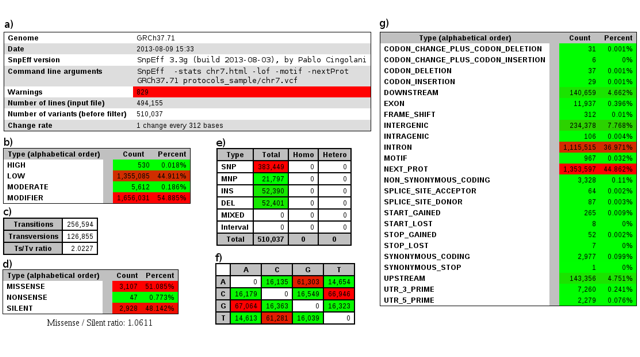
\includegraphics[width=14cm]{snpeff_1.png}
    \caption{Summary file produced by SpnEff. a) Overall summary showing input file, number of variants, command line, errors and warnings; b) number of impact assessed in each category; c) Transitions vs transversions; d) number of missense, nonsense and silent SNPs; e) number of variants by type (SNV, MNP, insertions, deletions and mixed); f) base change matrix; g) number of effects in each category.}
    \label{fig:snpeff1}
\end{figure}

\paragraph{Step 2. Counting variants in case and control subjects} In the first step of our protocol, SnpEff created a VCF file with half million annotated variants. Rather than scanning each annotation manually, we will use the SnpSift program to create a filter that will identify a small subset of variants with interesting functional properties. Since the VCF files used in most sequencing studies are even larger than the one in this example, our overall approach is to start by creating a filter using a very restrictive set of criteria. If no relevant variant is found using this stringent filter, we will relax the criteria to include variants with lower predicted impact.

In our example, since the pedigree is consistent with a Mendelian recessive disease, so we will first use SnpEff to find high impact variants that are homozygous in cases and either absent or heterozygous in controls. This provides a very strong genetic argument to select the promising variants and will be used as the first step in our filter. To do this, we will identify the case and control samples by providing SnpEff with pedigree information using a ``TFAM" file (a standard file format used to describe pedigrees). In our example, the TFAM file (\texttt{pedigree.tfam}) identifies the three cases (NA12879, NA12885, NA12886), and lists the other family members as controls. The \texttt{caseControl} command instructs the SnpSift program to count the number homozygous non-reference, heterozygous and allele count (number of non-reference alleles in each DNA sample) for both cases and controls groups (running time: $~60$ minutes):

\begin{lstlisting}[language=bash]
java -Xmx1g -jar SnpSift.jar \
       caseControl \
       -v -tfam protocols/pedigree.tfam protocols/ex1.eff.vcf \
       > protocols/ex1.eff.cc.vcf
\end{lstlisting}

This analysis creates an output VCF file (\texttt{ex1.eff.cc.vcf}) by adding new information to the \texttt{INFO} field for each variant: this includes information such as \texttt{Cases=1,1,3} and \texttt{Controls=8,6,22}, which correspond to the number of homozygous non-reference, heterozygous and total allele counts in cases and controls for each variant. The program also calculates basic statistics for each variant based on the allele frequencies in the two groups using different models, which can be useful as a starting point for more in-depth statistical analysis.

\paragraph{Step 3. Filtering variants} We can use the \texttt{SnpSift filter} command to reduce the number of candidate loci base on alleles in cases and controls. SnpSift \texttt{filter} allows users to create powerful filters that select variants using Boolean expressions containing data from the VCF fields. The expression we use to filter the VCF file \texttt{ex1.eff.vcf} is developed based on the expectation that all the three cases and none of the controls to be homozygous for the mutation. This is expressed using the following filter: \texttt{(Cases[0] = 3) \& (Controls[0] = 0)}. The full command line is:

\begin{lstlisting}[language=bash]
cat protocols/ex1.eff.cc.vcf \
    | java -jar SnpSift.jar filter \
         "(Cases[0] = 3) & (Controls[0] = 0)" \
    > protocols/ex1.filtered.hom.vcf
\end{lstlisting}

The filtered output file, \texttt{filtered.hom\_cases.vcf}, contains over 400 variants satisfying our criteria. This is still too large to analyze by hand, so can we can add another filter to see if any of these variants is expected to have a high impact. To identify variants where any of these impacts is classified as either \textit{HIGH} or \textit{MODERATE}, we add the condition \texttt{EFF[*].IMPACT = 'HIGH') | (EFF[*].IMPACT = 'MODERATE')}. The new filtering commands become:

\begin{lstlisting}[language=bash]
cat protocols/ex1.eff.cc.vcf \
    | java -jar SnpSift.jar filter \
            "(Cases[0] = 3) & (Controls[0] = 0) & ((EFF[*].IMPACT = 'HIGH') | (EFF[* ].IMPACT = 'MODERATE'))" \
    > protocols/ex1.filtered.vcf
\end{lstlisting}

After filtering, only two variants satisfy our criteria (Figure \ref{fig:snpefffilteredvars}), one of them is a \textit{STOP\_GAINED} loss of function variant, whereas the other one is a \textit{NON\_SYNONYMOUS} amino acid change. The first one is a known Cystic fibrosis variant.

\begin{figure}
    \centering
    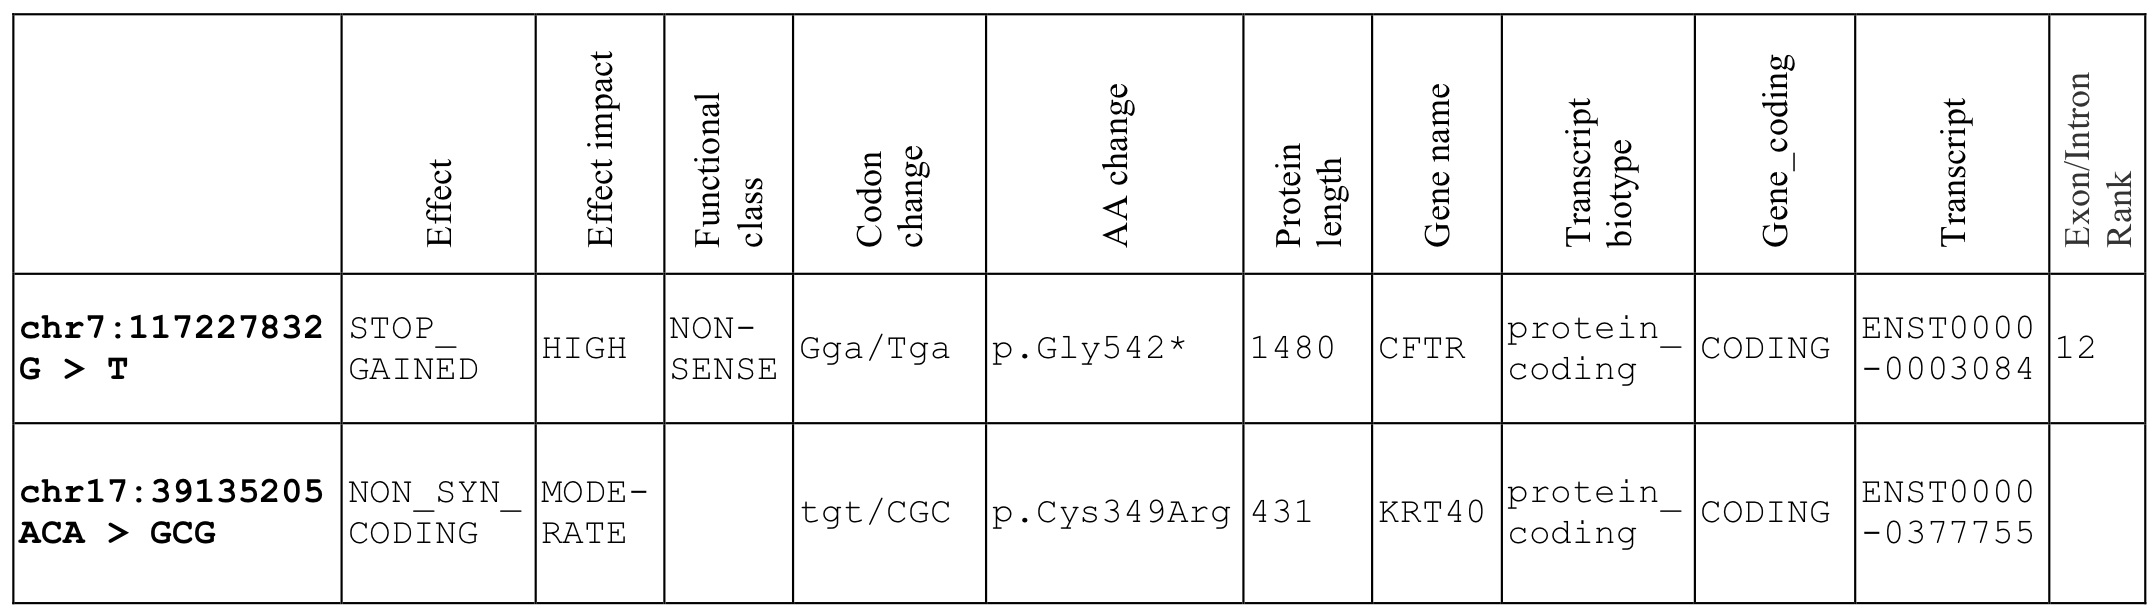
\includegraphics[width=14cm]{snpeff_table_variants_filtered.png}
    \caption{Candidate variants remaining after filtering.}
    \label{fig:snpefffilteredvars}
\end{figure}

A chart showing how the variant propagates across the pedigree structure (Figure \ref{fig:snpeff2}) can be created as follows:

\begin{lstlisting}[language=bash]
java -jar SnpSift.jar pedShow \
       protocols/pedigree.tfam protocols/ex1.filtered.vcf protocols/chart
\end{lstlisting}

\begin{figure}
    \centering
    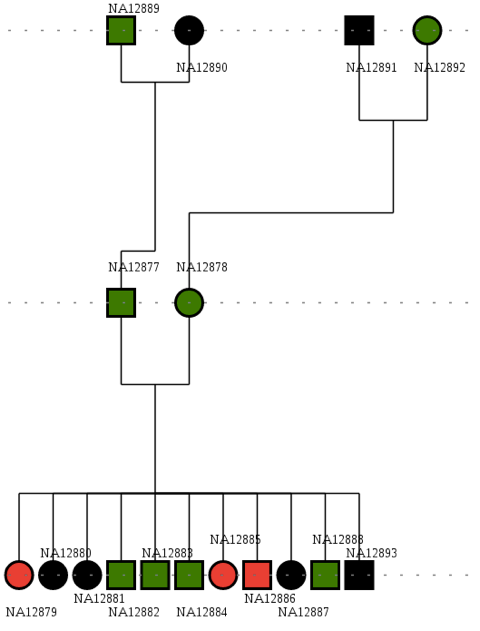
\includegraphics[width=8cm]{snpeff_2.png}
    \caption{Pedigree used for Procedure 1. A pedigree, created using the "SnpEff pedShow" command, shows heterozygous individuals in green, and homozygous alternative in red. It shows how the cystic fibrosis variant gets propagated from heterozygous unaffected grandparents and parents to homozygous affected offspring.}
    \label{fig:snpeff2}
\end{figure}

\paragraph{Step 4. Using clinical databases.} So far, since the purpose of the example was to show how annotations and filtering are performed to uncover new variants, we assumed that the causative variant was not known. In reality the variant is known and databases, such as ClinVar, have this information in convenient VCF format that can be used for annotations. We can annotate using ClinVar by using the following command:

\begin{lstlisting}[language=bash]
java -Xmx1g -jar SnpSift.jar annotate \
       -v protocols/db/clinvar_00-latest.vcf protocols/ex1.eff.cc.vcf \
       > protocols/ex1.eff.cc.clinvar.vcf
\end{lstlisting}

Our variant of interest is then annotated as \textit{``Cystic Fibrosis"} (to find the variant, we filter for variants having ClinVar annotation \textit{``CLNDBN"} that are in CFTR gene and have a \textit{STOP\_CODON} annotation):

\begin{lstlisting}[language=bash]
cat protocols/ex1.eff.cc.clinvar.vcf | java -jar SnpSift.jar filter \
     "(exists CLNDBN) & (EFF[*].EFFECT = 'STOP_GAINED') & (EFF[*].GENE = 'CF TR')"
\end{lstlisting}

\paragraph{Software Integration (Optional)} Sequence analysis software is often run in high performance computers combining several programs into processing pipelines. Annotations and impact assessment software needs to provide integration points with other analysis steps of the pipeline. In the following paragraphs we describe how to integrate SnpEff with two programs commonly used in sequencing analysis pipelines: i) Genome Analysis toolkit (GATK 2), a command-line driven software; and ii) Galaxy 3, a web based software.

\paragraph{GATK} The Genome Analysis Toolkit 2 is one of the most popular programs for bioinformatics pipelines. Annotations can be easily integrated into GATK using SnpEff and GATK’s VariantAnnotator module. Here we show how to annotate a file using SnpEff and GATK, as an alternative way of performing step 1. You should perform this step only if your processing pipeline is based on GATK: compared to running SnpEff from the command line, the results obtained when using GATK will only contain the highest impact annotation for each variant. This was a conscious trade-off made by the designers of GATK, partly because most biologists do this implicitly when reading a list of variants, but also to improve the readability and reduce the size of the annotation results.

The method requires two steps: i) Annotating a VCF file using SnpEff and ii) using GATK’s VariantAnnotator to incorporate those annotations into the final VCF file. When using SnpEff for GATK compatibility, we must use the \texttt{-o gatk} command line option:

\begin{lstlisting}[language=bash]
java -Xmx4g -jar snpEff.jar -v \
       -o gatk GRCh37.75 protocols/ex1.vcf \
       > protocols/ex1.eff.gatk.vcf
\end{lstlisting}

Next, we process these variants using GATK. For this step to work correctly, we need to make sure that our data files are compatible with the requirements GATK places on reference genomes (see GATK’s documentation for more details): (i) in the fasta file, chromosomes are expected to be sorted in karyotypic order; (ii) a genome fasta-index file must be available; and (iii) a dictionary file must be pre-computed. Assuming these requirements are satisfied, we can run the following command, which will produce a GATK annotated file (\texttt{ex1.gatk.vcf}):

\begin{lstlisting}[language=bash]
java -Xmx4g -jar $HOME/tools/gatk/GenomeAnalysisTK.jar \
       -T VariantAnnotator \
       -R $HOME/genomes/GRCh37.75.fa \
       -A SnpEff \
       --variant protocols/ex1.vcf \
       --snpEffFile protocols/ex1.eff.gatk.vcf \
       -L protocols/ex1.vcf \
       -o protocols/ex1.gatk.vcf
\end{lstlisting}

Note: We assumed GATK is installed in \texttt{\$HOME/tools/gatk/} and the reference genome is contained in \texttt{\$HOME/genomes/GRCh37.75.fa}. These file locations should be adapted to the actual path in your computer.

\paragraph{Galaxy} Another popular tool in bioinformatics is Galaxy 3, which allows pipelines to be created in a web environment using graphical interface, making it flexible and straightforward to use. SnpEff provides Galaxy modules (see http://snpeff.sourceforge.net/SnpEff\_manual.html\#galaxy for details). Once these modules are installed, we can run our sample annotation pipeline in Galaxy (Figure \ref{fig:snpeff3}). A step-by-step tutorial can be found at http://snpeff.sourceforge.net/protocol

\begin{figure}
    \centering
    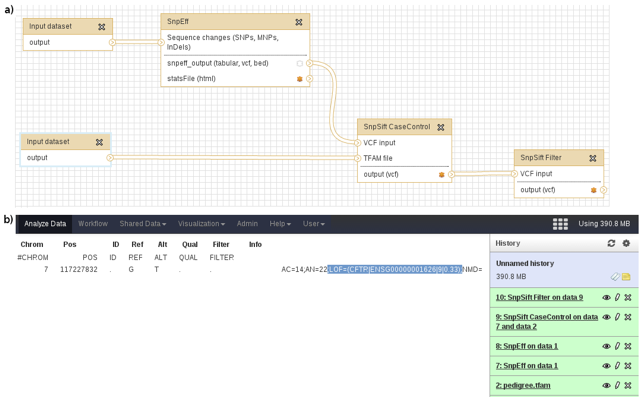
\includegraphics[width=14cm]{snpeff_3.png}
    \caption{Use of Galaxy combined with SnpEff. (a) Galaxy Protocol for example 1. Galaxy automatically creates a pipeline showing the processing steps, which can be modified and later used to process new datasets; (b) Results after the last step was executed by Galaxy server.}
    \label{fig:snpeff3}
\end{figure}

%---
\section{Procedure II: Analysis of non-coding variants}
%---

This example shows how to perform basic annotation of non-coding variants. It is based on a short list of 20 non-coding that were identified by sequencing a 700 kb region surrounding the gene T-box transcription factor (TBX5) in 260 patients with congenital heart disease 67. TBX5 is a transcription factor that plays a well-established dosage-dependent role in heart and limb development. Coding mutations in TBX5 have been frequently identified in patients with Holt–Oram syndrome, which is associated with abnormal hand, forearm and cardiac development.

\paragraph{Step 1. Annotating variants} We will perform non-coding variant annotation using SnpEff following a similar approach to Procedure I. In this case, we construct a command line that instructs SnpEff to include motif information (\texttt{-motif}) and putative transcription factor binding sites (TFBS) identified in the ENSEMBL Regulatory Build and the Jaspar database:

\begin{lstlisting}[language=bash]
java -Xmx4g -jar snpEff.jar -v \
       -motif GRCh37.75 protocols/ex2.vcf \
       > protocols/ex2.eff.basic.vcf
\end{lstlisting}

\paragraph{Step 2. Adding custom regulatory information} A quick scan through the results shows that most variants are catalogued as \textit{INTERGENIC}, and none of them is associated with a known TFBS. This is not surprising since TFBS are small and also because regulatory elements involved in cardiac or limb development may not be widely active in commonly studied adult tissues. In this case, basic annotations did not provide additional information that can be used to narrow down the list of candidate SNVs. To solve this, the authors examined data from other sources, including ChIP-seq data for H3K4me1 (a post-translationally modified histone protein found in transcriptionally active genome regions, including enhancers and promoters). Data produced from ChIP-Seq analysis are frequently published in BED, BigBed or similar formats, which can be used directly by SnpEff by adding the ``-interval" command line option. This command line option can be used to add annotations using ChIP-Seq experiments from the ENCODE and Epigenome Roadmap projects: since multiple ``-interval" options are allowed in each command line, it is a simple way to combine several annotations:

\begin{lstlisting}[language=bash]
java -Xmx4g -jar snpEff.jar -v \
       -motif -interval protocols/ex2_regulatory.bed GRCh37.75 \
       protocols/ex2.vcf \
       > protocols/ex2.eff.vcf
\end{lstlisting}

In the output VCF file, variants intersecting genomic regions from the \texttt{-interval} command line option are annotated as \texttt{CUSTOM[ex2\_regulatory]} : the name in brackets identifies the file name provided to distinguish multiple annotation files.

\paragraph{Step 3. Adding conservation information} In order to refine our search, we can also look for variants in highly conserved non-coding bases. SnpEff natively supports PhastCons scores, but can also add annotations based on any other user-defined score provided as a Wig or VCF file. The command line for annotating using the PhastCons score is:

\begin{lstlisting}[language=bash]
java -Xmx1g -jar SnpSift.jar \
      phastCons -v protocols/phastcons protocols/ex2.eff.vcf \
      > protocols/ex2.eff.cons.vcf
\end{lstlisting}

Now we can filter our results looking for a highly conserved SNP in the regulatory region. We do this by using a \texttt{SnpSift filter} command and the appropriate Boolean expression:

\begin{lstlisting}[language=bash]
cat protocols/ex2.eff.cons.vcf \
    | java -jar SnpSift.jar filter \
            "(EFF[*].EFFECT = 'CUSTOM[ex2_regulatory]') & (exists PhastCons) & (PhastC ons > 0.9)" \
    > protocols/ex2.filtered.vcf
\end{lstlisting}

SnpSift \texttt{filter} supports a flexible syntax to create Boolean expressions using the annotation data that provides a versatile way to prioritize shorter lists of SNPs for subsequent validation. This syntax is described in detail in the online manual (http://snpeff.sourceforge.net/SnpSift.html\#filter). In this example, our filter results in only two candidate SNPs, one of which was extensively validated in the original study and is assumed to be causative 67.

The principles illustrated in our example for a small set of SNVs can be applied to millions of variants from whole genome sequencing experiments. Similarly, although we filtered the SNVs using \texttt{custom} ChIP-seq data that provided in the original study 67, regulatory information from public Encode or Epigenome Roadmap datasets could be used in a first line investigation before generating our own Chip- seq or RNA-seq data using disease-relevant cells and tissues.

\section{Troubleshooting}

Complete documentation for SnpEff, together with troubleshooting instructions are available at http://snpeff.sourceforge.net/SnpEff\_manual.html.

\section{Acknowledgements}

We thank Louis Létourneau and Adrian Platts, for their valuable suggestions for improving SnpEff. This work was funded by the National Institute of Diabetes \& Digestive \& Kidney diseases (NIDDK 5-U01- DK085545-02) and the Canadian Institutes for Health Research (CIHR MOP-102703).
